\chapter{Design suppliments}
\label{appendix:sup_design}

\section{CRC cards}\label{sup:crc}
Below is an excerpt of the the examples of a more complex CRC card design in the system. Throughout the the project, each class went through an iterative process of using CRC cards. Therefore, a lot of them have been omitted to save space.

\begin{figure}[H]
  \centering
  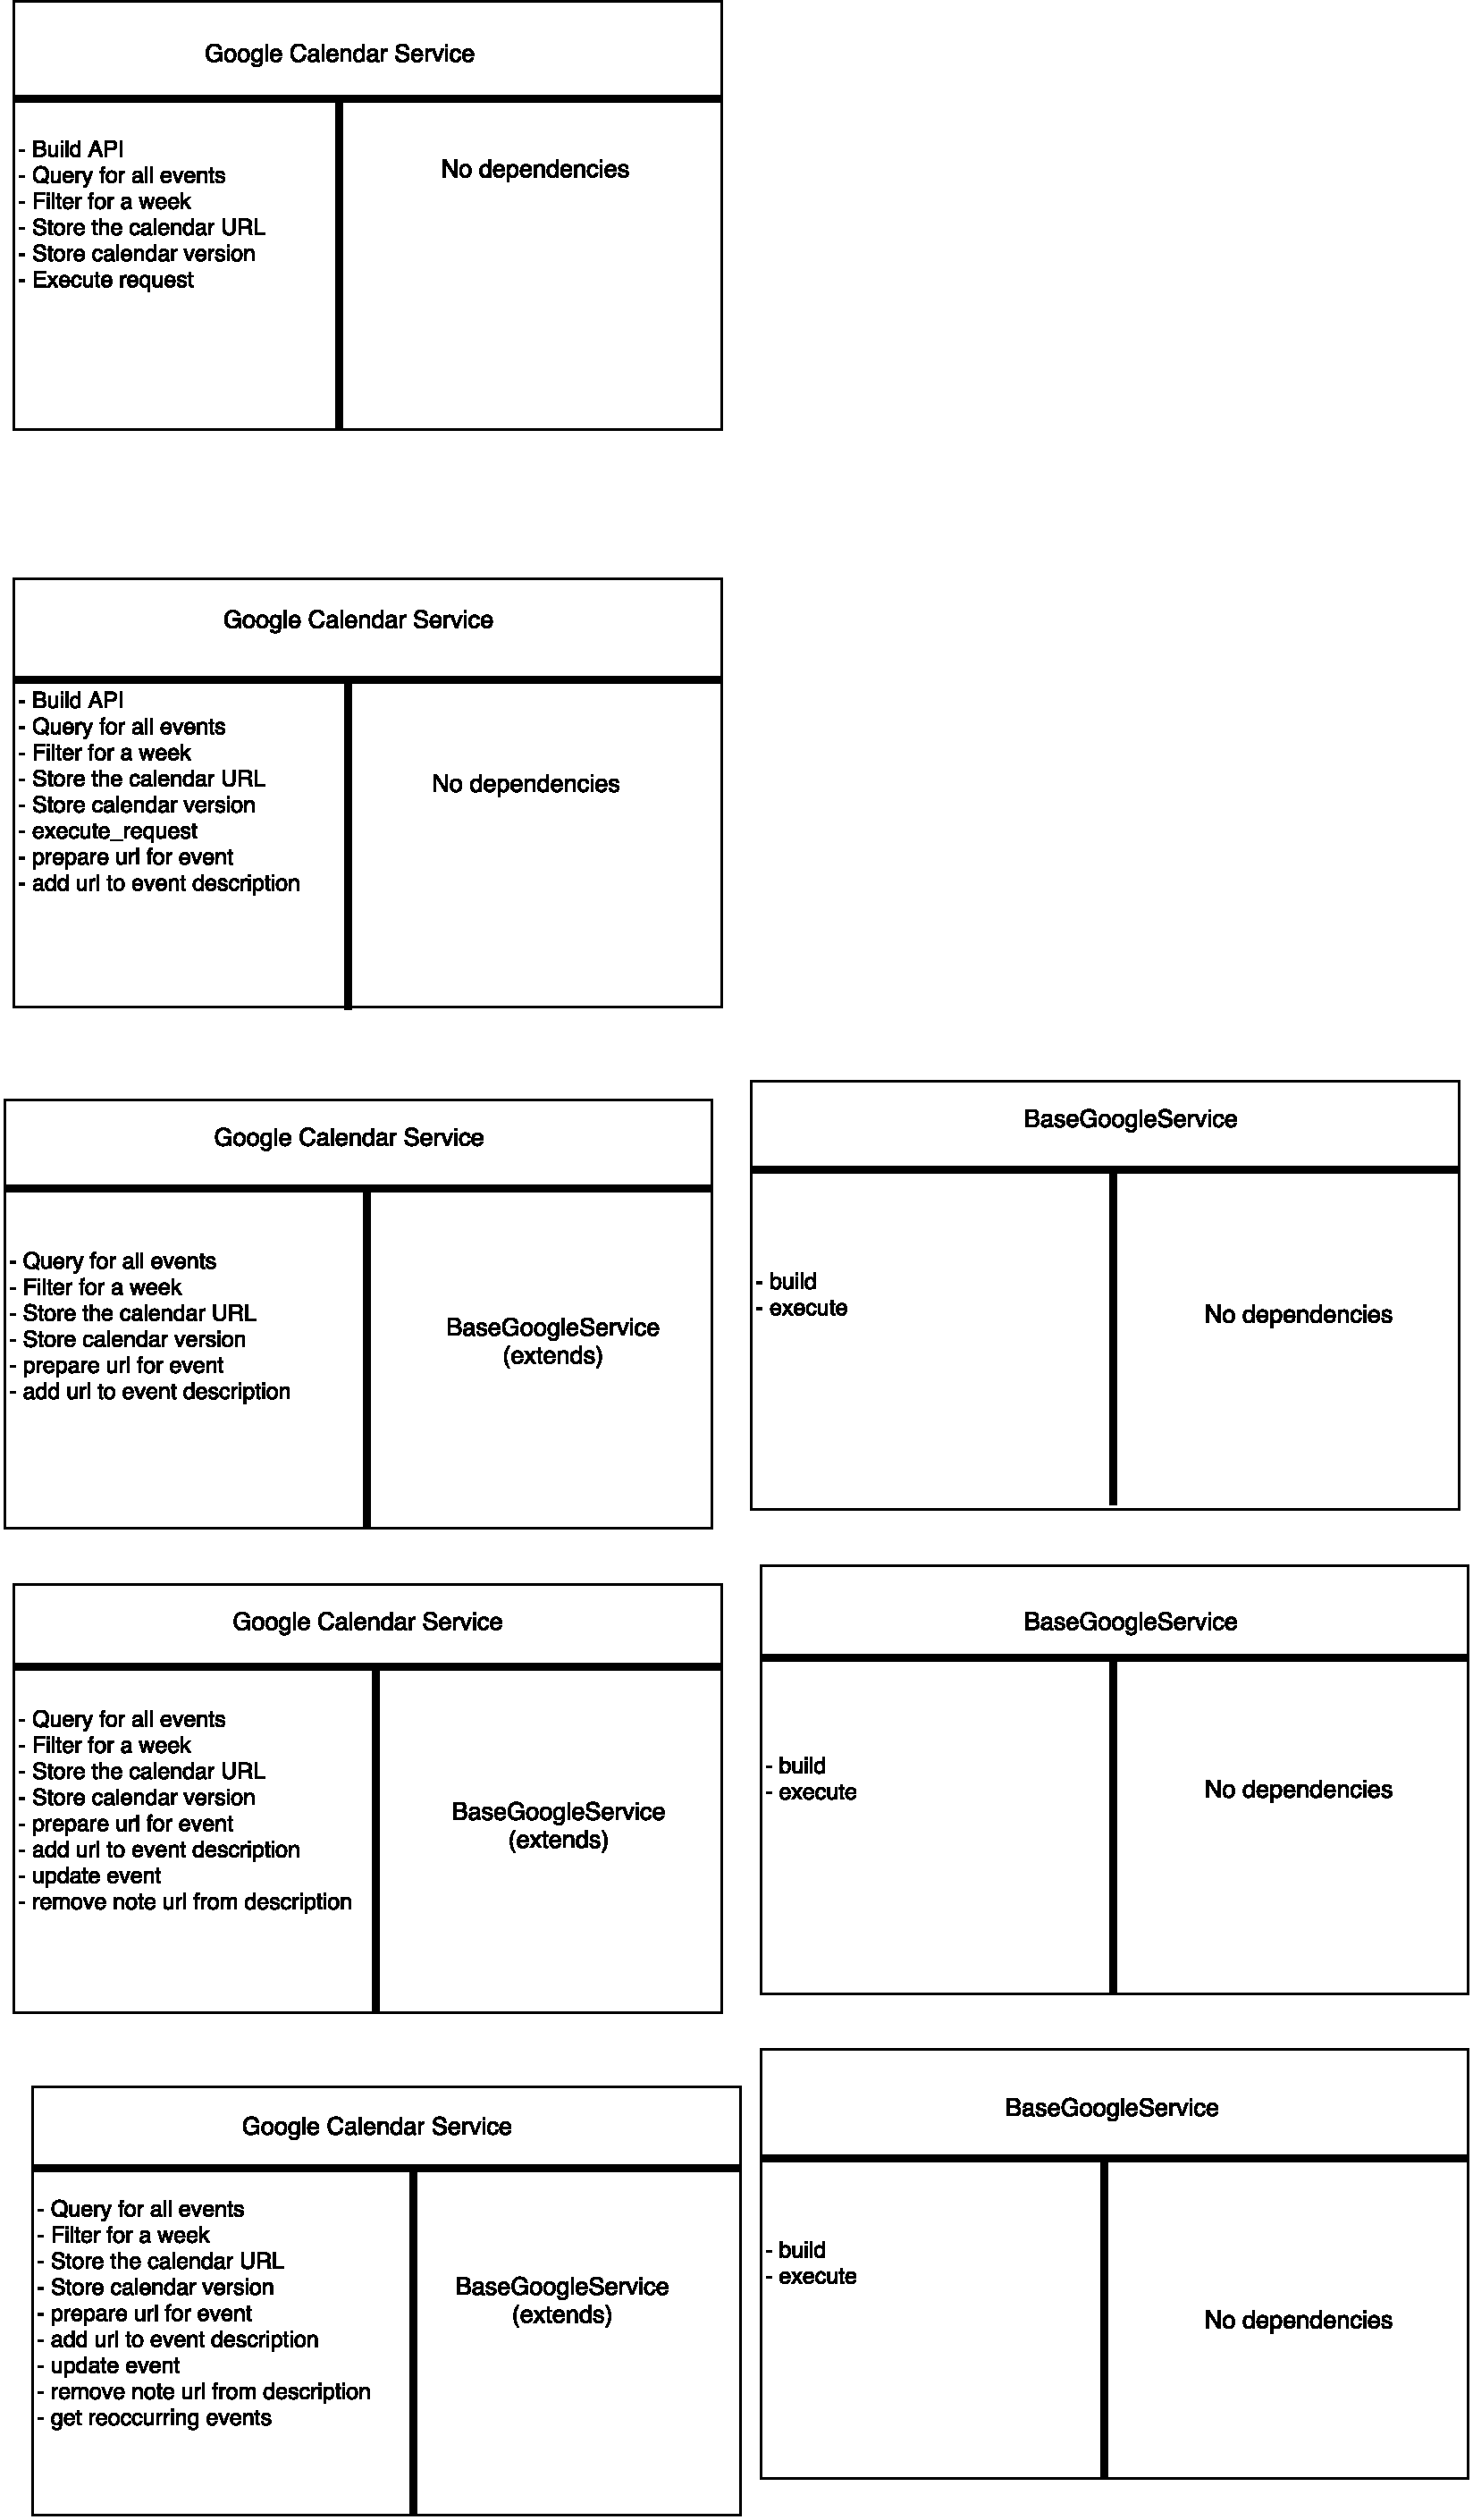
\includegraphics{images/google_calendar_service.pdf}
  \label{fig:crc_card_google_calendar}
  \caption{An iterative approach to the CRC cards, used in the design of the Google calendar service. Each now card represents a new state in which the system has evolved.}
\end{figure}

\section{Wireframes} \label{sup:wireframe}
\begin{figure}[H]
  \centering
  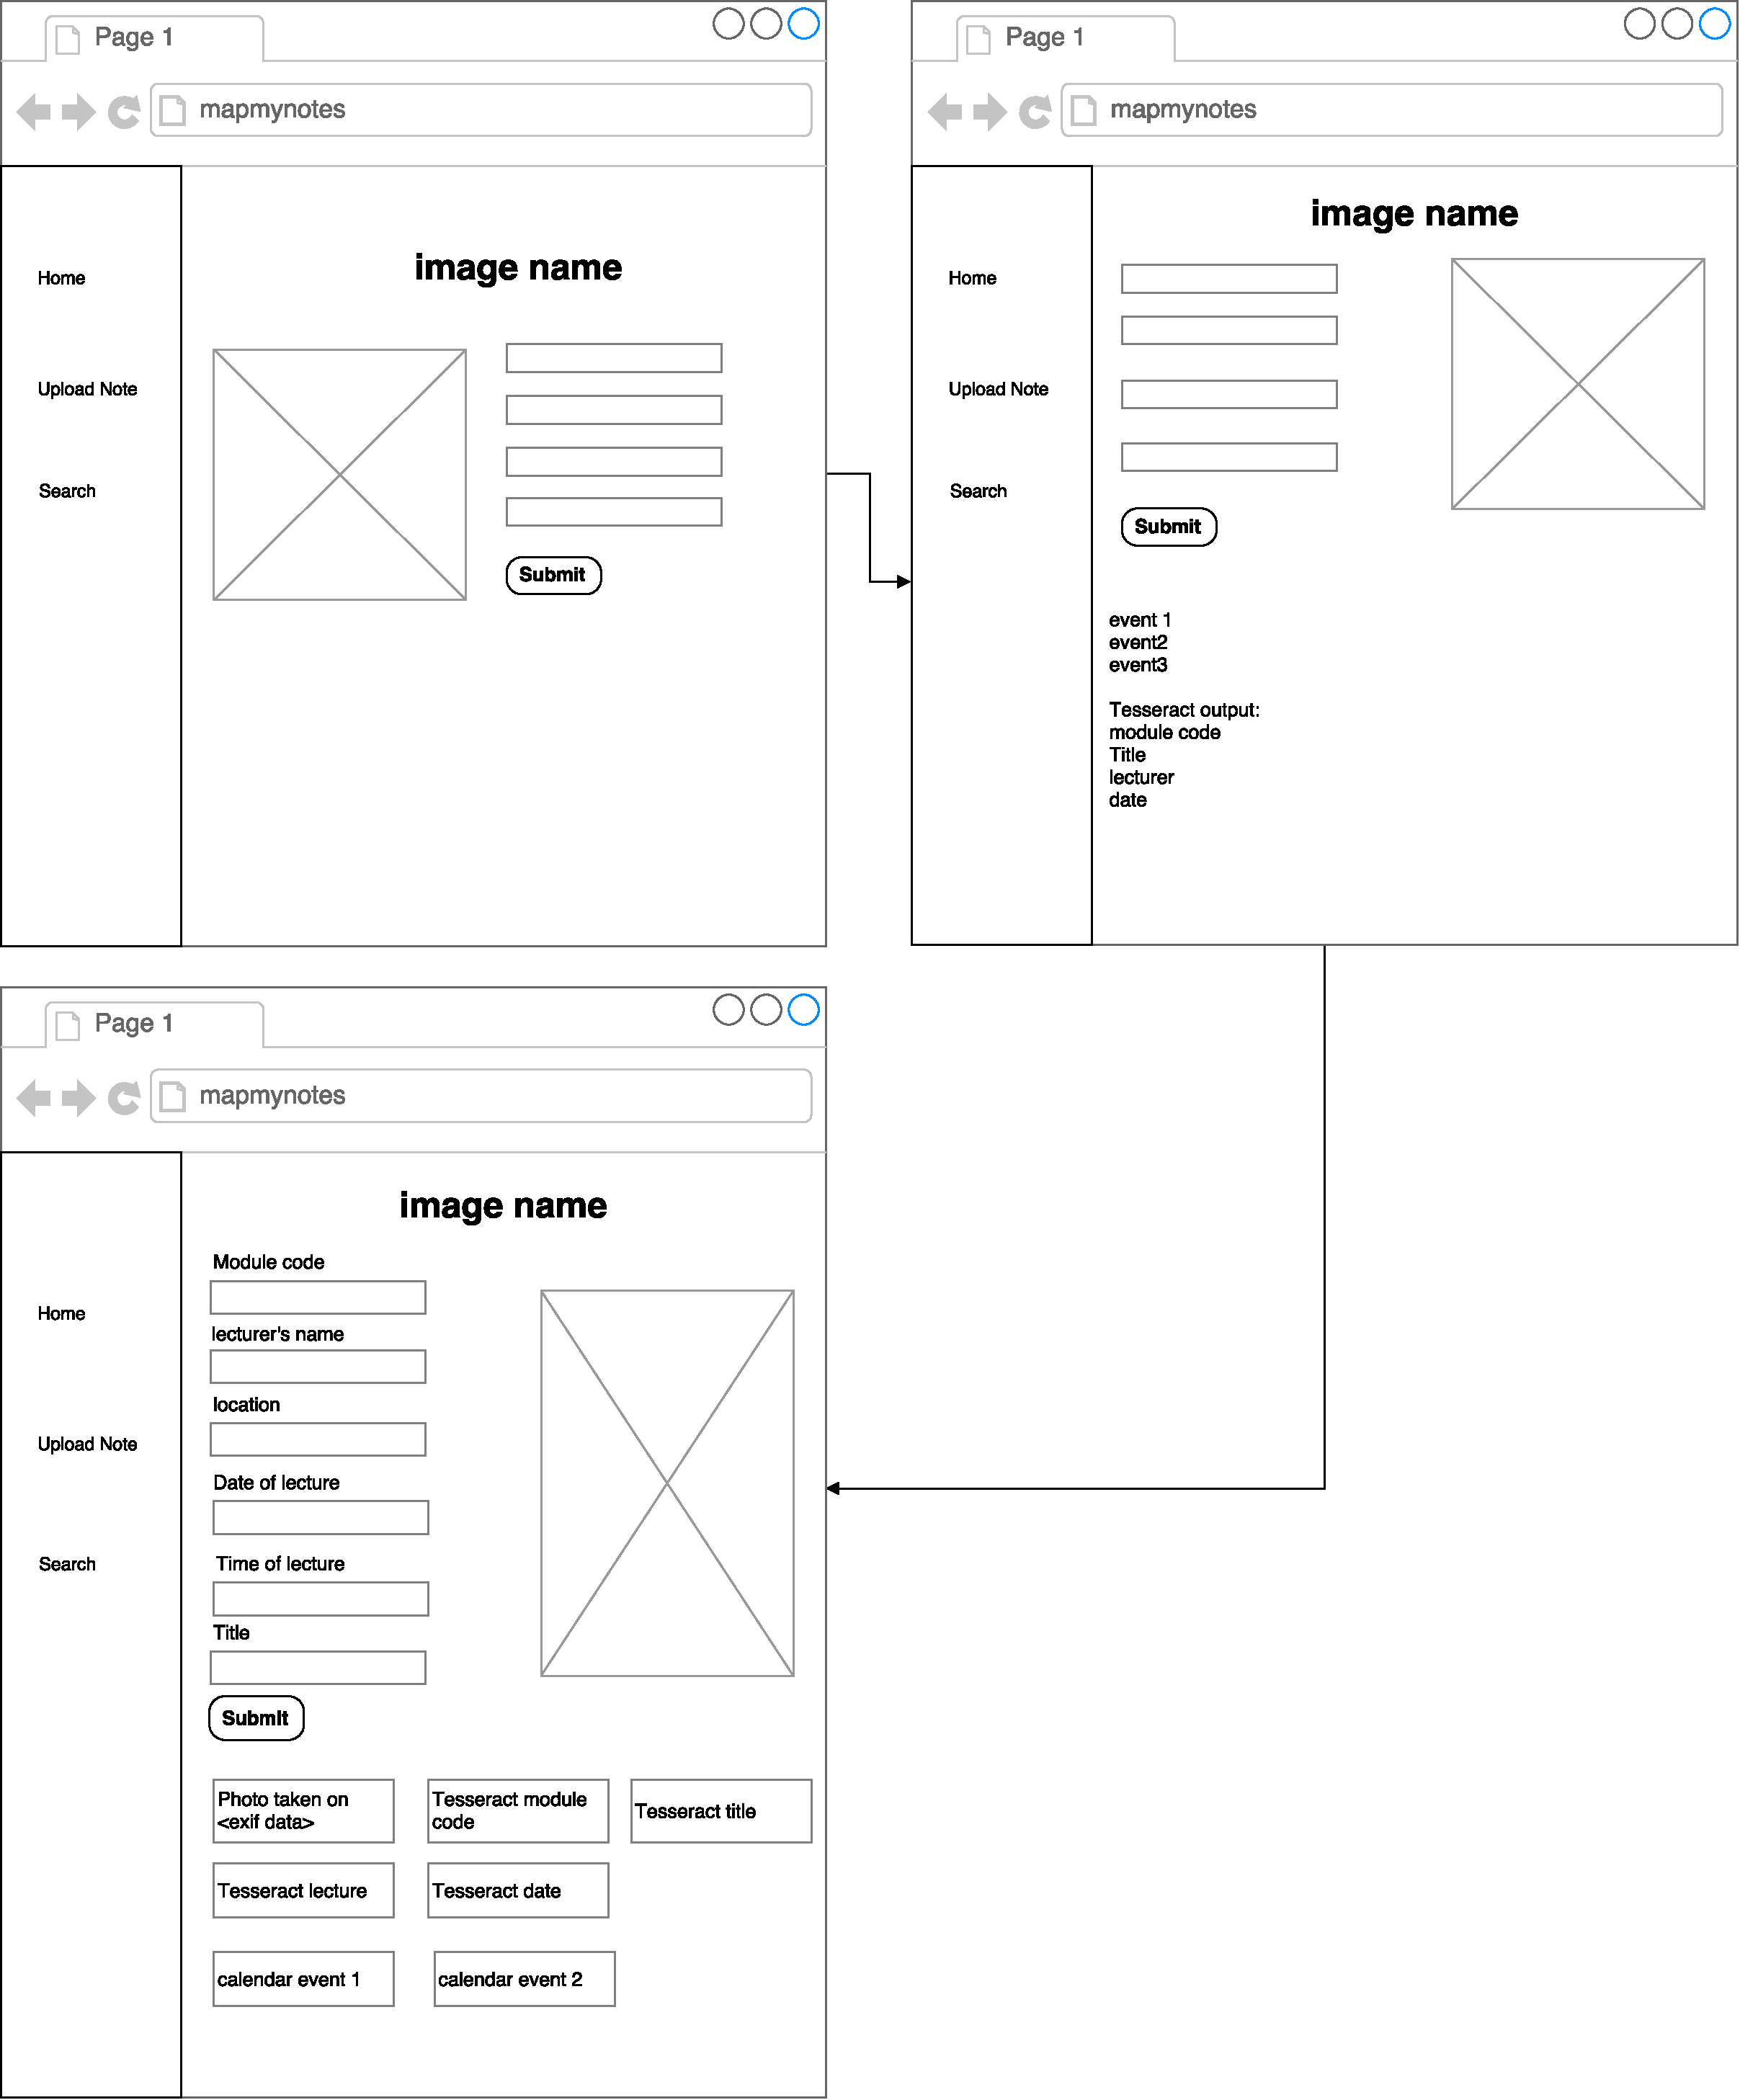
\includegraphics{images/upload_note_wire_frame.pdf}
  \label{fig:note_wire_frame}
  \caption{An example of progressive wireframes for the note upload leading to an overall design which could be implemented for the end user. }
\end{figure}
